\section{Results and analysis}\label{sec:results}

\subsection{Forecast quality}

Table~\ref{tab:main} reports forecast quality on the unseen wells with fixed hyper-parameters; the tuned
counterparts are in Appendix~\ref{app:extra} (Table~\ref{tab:tuned}). Three groups emerge. The physics
rule B0 ranks windows reasonably (AUROC 0.83) but is badly calibrated (ECE 0.66) and catches no event under
a deployed threshold; logistic regression and the autoencoder detector B9 perform below chance level on
AUROC, which shows that an anomaly score is not a forecast of time to a critical state. The recurrent and
convolutional forecasters form the strongest group: the LSTM reaches the highest AUPRC@24h ($0.736\pm0.066$
over three seeds), and the GRU, CNN-LSTM, TCN and Transformer--LSTM lie within one standard deviation of it
(0.69--0.71). PI-PatchSurv reaches $0.644\pm0.055$ over five seeds and AUROC $0.794\pm0.018$, below the
recurrent group on ranking but with the lowest seed-to-seed spread in AUROC.

The precision--recall curves in Figure~\ref{fig:pr} explain part of the difference between mean-of-folds
and pooled AUPRC. When the test wells are pooled, PI-PatchSurv keeps higher precision at low recall than
the recurrent models (pooled AUPRC 0.54 versus 0.45 for the LSTM), because its scores are more comparable
across wells; the per-fold mean, which averages within-well rankings, favours the recurrent models. All
deep models clearly exceed the prevalence of 0.14.

\begin{table*}[t]
\caption{Forecast quality on unseen wells (six leave-one-well-out folds, 24 events), fixed hyper-parameters}\label{tab:main}
\scriptsize\setlength{\tabcolsep}{3pt}
\resizebox{\textwidth}{!}{\begin{tabular}{lcccccccccc}
\toprule
Model & Seeds & AUPRC@24h & AUROC@24h & C-index & IBS & ECE & BSS & Rec.@1/mo & Hits/24 & PICP \\
\midrule
{B0 $\widetilde{\mathrm{RI}}^*$ rule} & 1 & 0.533 & 0.828 & 0.819 & 0.728 & 0.658 & 0.00 & 0.00 & 0 & -- \\
{B1 Logistic regression} & 1 & 0.281 & 0.406 & 0.434 & 0.366 & 0.529 & 0.26 & 0.04 & 0 & 0.94 \\
{B2 GBDT} & 1 & 0.679 & 0.892 & 0.811 & 0.088 & 0.226 & 0.67 & 0.62 & 4 & 0.72 \\
{B3 LSTM} & 3 & 0.736$\pm$0.066 & 0.910$\pm$0.038 & 0.869 & 0.078 & 0.177 & 0.80 & 0.62 & 4.7$\pm$3.1 & 0.54 \\
{B4 GRU} & 3 & 0.712$\pm$0.123 & 0.905$\pm$0.061 & 0.889 & 0.094 & 0.204 & 0.78 & 0.67 & 14.7$\pm$1.5 & 0.43 \\
{B5 CNN-LSTM} & 3 & 0.708$\pm$0.122 & 0.893$\pm$0.095 & 0.863 & 0.121 & 0.258 & 0.70 & 0.71 & 6.3$\pm$4.2 & 0.29 \\
{B6 TCN} & 3 & 0.687$\pm$0.060 & 0.919$\pm$0.028 & 0.847 & 0.089 & 0.179 & 0.78 & 0.67 & 4.3$\pm$5.8 & 0.61 \\
{B7 Transformer-LSTM$^\dagger$} & 3 & 0.711$\pm$0.031 & 0.903$\pm$0.058 & 0.889 & 0.087 & 0.174 & 0.82 & 0.67 & 13.7$\pm$0.6 & 0.33 \\
{B8 PatchTST$^\dagger$} & 3 & 0.569$\pm$0.041 & 0.807$\pm$0.032 & 0.792 & 0.101 & 0.137 & 0.81 & 0.79 & 2.0$\pm$1.0 & 0.52 \\
{B8i iTransformer} & 3 & 0.633$\pm$0.047 & 0.855$\pm$0.074 & 0.782 & 0.083 & 0.132 & 0.75 & 0.21 & 6.0$\pm$7.0 & 0.88 \\
{B9 LSTM-AE detector$^\dagger$} & 1 & 0.262 & 0.365 & 0.478 & 0.749 & 0.849 & -0.96 & 0.00 & 0 & 0.81 \\
\textbf{PI-PatchSurv (proposed)} & 5 & 0.644$\pm$0.055 & 0.794$\pm$0.018 & 0.802 & 0.103 & 0.234 & 0.69 & 0.25 & 5.8$\pm$2.9 & 0.87 \\
\bottomrule
\end{tabular}}
\footnotetext{AUPRC/AUROC and hits: mean$\pm$SD over single-seed runs where several seeds exist; other columns: ensemble of the available seeds. BSS: Brier skill score at 24~h relative to B0. Rec.@1/mo: threshold-free recall at one false alarm per well-month. Hits: events caught out of 24 with the deployed calib-self threshold. PICP: coverage of the 90\,\% conformal interval. $^\dagger$Re-implementation of a base-paper architecture.}
\end{table*}


\begin{figure*}[t]
\centering
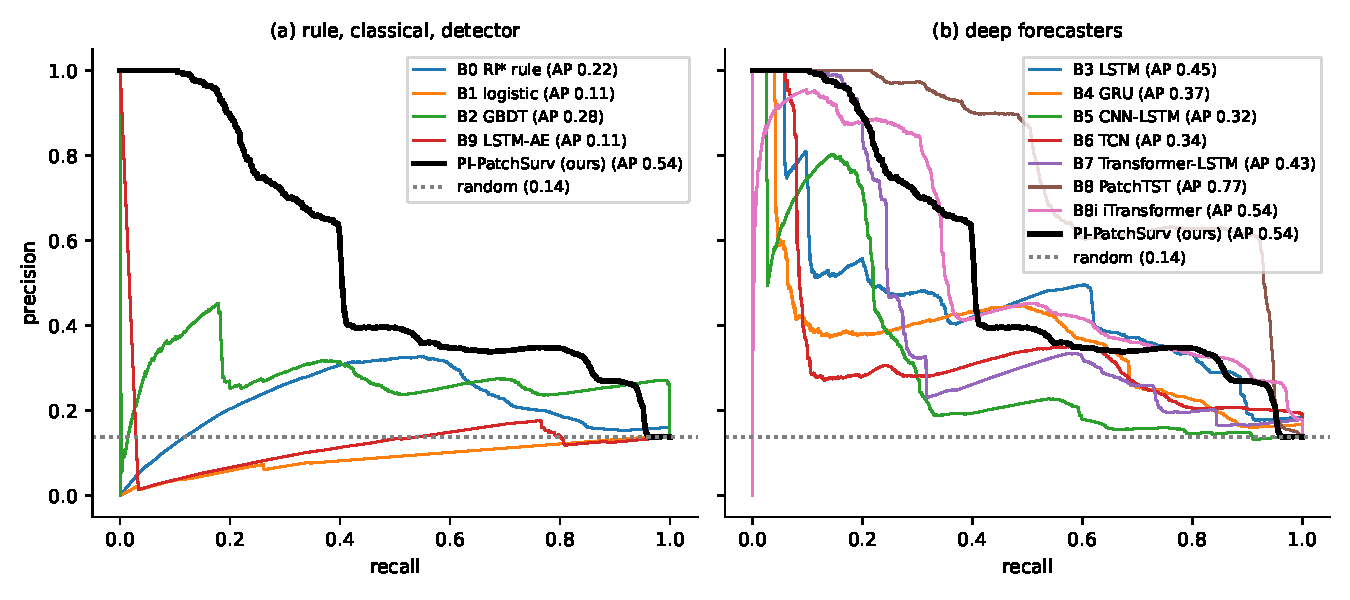
\includegraphics[width=\textwidth]{figures/pr_curves_24h.pdf}
\caption{Precision--recall curves for an event within 24~h, pooled over the six test wells (ensemble of the
available seeds). (a) Physics rule, classical learners and the autoencoder detector; (b) deep forecasters.
The dotted line is the event prevalence.}
\label{fig:pr}
\end{figure*}

\subsection{Deployed alarms}

Ranking does not guarantee a useful alarm, because the threshold has to be fixed before the test well is
seen. Table~\ref{tab:alarms} reports alarms with thresholds chosen on the calibration wells for at most one
false alarm per well-month. With the raw score (\emph{calib}) most models either miss events or raise many
false alarms on the new well, since absolute score levels differ between wells. Subtracting each
instance's own first-hour score (\emph{calib-self}) corrects much of this shift for the recurrent models:
the GRU ensemble improves from 8 to 15 events caught, and the Transformer--LSTM keeps 13--15 events while
its false-alarm rate falls from 0.24 to 0.044 per well-day. For PI-PatchSurv the correction hurts (15 events at
0.26 false alarms per well-day with the raw score, 9 at 0.19 with calib-self). Over seeds, the GRU catches
$14.7\pm1.5$ events at $0.054\pm0.006$ false alarms per well-day and the Transformer--LSTM $13.7\pm0.6$ at
$0.040\pm0.012$; the best single run (tuned GRU) catches 17 of 24 events at 0.052 per well-day with an event
precision of 0.57 and a median lead of 2.9~h. These rates correspond to about 1.2--1.6 false alarms per
well-month, close to but above the target of one. PI-PatchSurv catches $5.8\pm2.9$ events: its score drifts
within the long well-24 instances, which the self-referenced threshold converts into false alarms
(Appendix~\ref{app:extra}). No model false-alarms on the class-6 look-alike (quick restriction of the
choke); hydrate events (classes 8 and 9) are the main confounder, because a downstream plug also raises the
upstream pressure slowly (Table~\ref{tab:faclass}).

\begin{table*}[t]
\caption{Deployed alarms with thresholds fixed on the calibration wells (ensemble of the available seeds; 24 events, about 248 negative well-days). FA: false alarms per negative well-day}\label{tab:alarms}
\footnotesize
\resizebox{\textwidth}{!}{\begin{tabular}{lcccccc}
\toprule
 & \multicolumn{2}{c}{Raw score (calib)} & \multicolumn{4}{c}{Self-referenced score (calib-self)} \\
\cmidrule{2-3}\cmidrule{4-7}
Model & Hits/24 & FA & Hits/24 & FA & Event precision & Lead, h: median (IQR) \\
\midrule
B2 GBDT & 1 & 0.335 & 4 & 0.262 & 0.06 & 31.5 (29.2) \\
B3 LSTM & 17 & 0.254 & 9 & 0.044 & 0.45 & 3.5 (3.6) \\
B4 GRU & 8 & 0.048 & 15 & 0.057 & 0.52 & 3.3 (2.3) \\
B4 GRU (tuned) & 17 & 0.258 & 17 & 0.052 & 0.57 & 2.9 (5.8) \\
B6 TCN & 2 & 0.242 & 1 & 0.073 & 0.05 & 1.3 (0.0) \\
B7 Transformer-LSTM & 13 & 0.238 & 15 & 0.044 & 0.58 & 1.8 (3.5) \\
B7 Transformer-LSTM (tuned) & 10 & 0.077 & 16 & 0.044 & 0.59 & 4.1 (4.4) \\
B8 PatchTST & 19 & 0.214 & 2 & 0.048 & 0.14 & 9.8 (7.7) \\
B8i iTransformer (tuned) & 15 & 0.061 & 14 & 0.105 & 0.35 & 4.7 (4.6) \\
PI-PatchSurv & 15 & 0.262 & 9 & 0.190 & 0.16 & 4.2 (37.1) \\
PI-PatchSurv (tuned) & 14 & 0.198 & 6 & 0.109 & 0.18 & 35.6 (51.3) \\
\bottomrule
\end{tabular}}
\end{table*}


\subsection{Calibration, uncertainty and horizon}

PI-PatchSurv provides the most reliable uncertainty. Its 90\,\% conformal intervals cover 87\,\% of the
test event windows and its median time-to-event error is $\Delta T=6.8$~h, whereas the recurrent models
under-cover (LSTM 0.54, GRU 0.43, Transformer--LSTM 0.33) with $\Delta T$ of 9--24~h; only the
iTransformer reaches similar coverage (0.88) with a larger error (10.0~h). The reliability diagram
(Appendix, Figure~\ref{fig:reliab}) shows that all models over-estimate risk above 0.6, which is expected
when the calibration well holds only one to three events. Figure~\ref{fig:horizon} shows that AUPRC rises
with the horizon for every model, from 0.02--0.33 at 1~h to 0.78--0.93 at 72~h: most windows lie within
a few days of their event, so long horizons are easier, and the short pre-onset records of 3W (median
6.5~h of normal data) cap the useful lead at a few hours.

\begin{figure}[t]
\centering
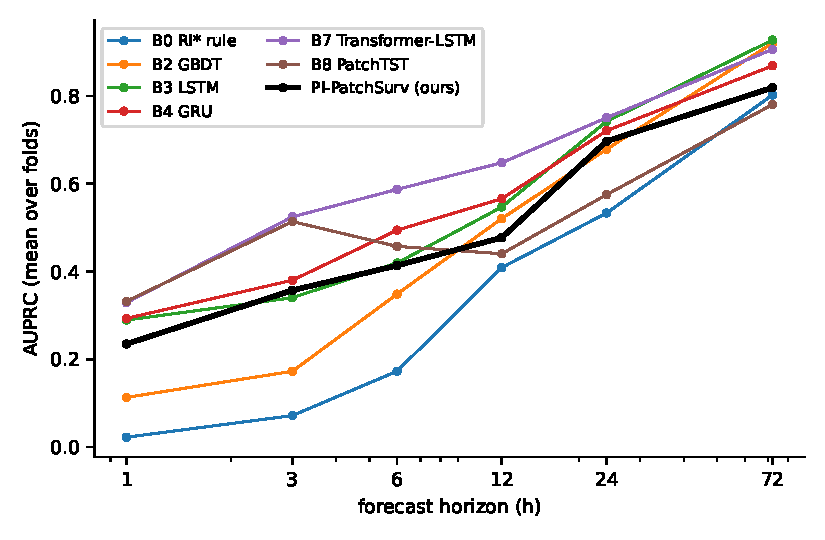
\includegraphics[width=\columnwidth]{figures/horizon_auprc.pdf}
\caption{Horizon sensitivity (E5): AUPRC (mean over folds) against the forecast horizon.}
\label{fig:horizon}
\end{figure}

\subsection{Robustness and generalisation}

Corruptions applied to the test inputs (Appendix~\ref{app:extra}, Table~\ref{tab:robust}) show a clear contrast. PI-PatchSurv is insensitive to sensor loss:
with three of nine sensors replaced by their median and flagged as missing its AUPRC is unchanged
(0.70), whereas the LSTM falls from 0.81 to 0.56 ($-30\,\%$). This follows from the channel-independent,
mask-aware design and is relevant because sensor failure is common in the field. Gaussian noise of up to
5\,\% and an undetected frozen sensor change neither model much. The LSTM is more robust to a change of the
sampling rate (30~s to 5~min, models not retrained) than PI-PatchSurv, whose patch length is tied to the
1-minute grid. In the v1$\to$v2 generalisation test (Appendix~\ref{app:extra}, Table~\ref{tab:v1v2}), where only four events are
available for training, the patch encoder without physics (PatchTST) transfers best (AUPRC 0.61, AUROC
0.92) and PI-PatchSurv reaches 0.28 (AUROC 0.84); the GRU catches 9 of 20 events at 0.05 false alarms per
well-day.


\subsection{Statistical significance}

A Friedman test over the five folds with events is borderline for both the fixed models
($\chi^2=18.2$, $p=0.08$) and the tuned models ($p=0.06$); the Nemenyi critical difference for twelve
models and five folds is 7.45 ranks, and no pair of models differs. Paired instance-level bootstraps with
Holm correction confirm only that PI-PatchSurv outperforms the physics rule, logistic regression and the
autoencoder detector (all $p<0.001$); no difference among the deep forecasters survives correction. With 24
events, 17 of them in one well, the deep models cannot be ranked with confidence, and we do not claim a
winner among them.

\subsection{Qualitative examples}

Figure~\ref{fig:examples} shows two test instances. On the fast-scaling well 24 both PI-PatchSurv and the
GRU follow $\RI$, drop when the restriction temporarily falls after half a day, and rise again before $t_E$.
On the slow-scaling well 22, $\RI$ oscillates for six days; the risk of PI-PatchSurv climbs steadily from
about 0.2 to 0.75, tracking the slow growth, while the GRU switches abruptly from low to high risk about
three days before the event.

\begin{figure*}[t]
\centering
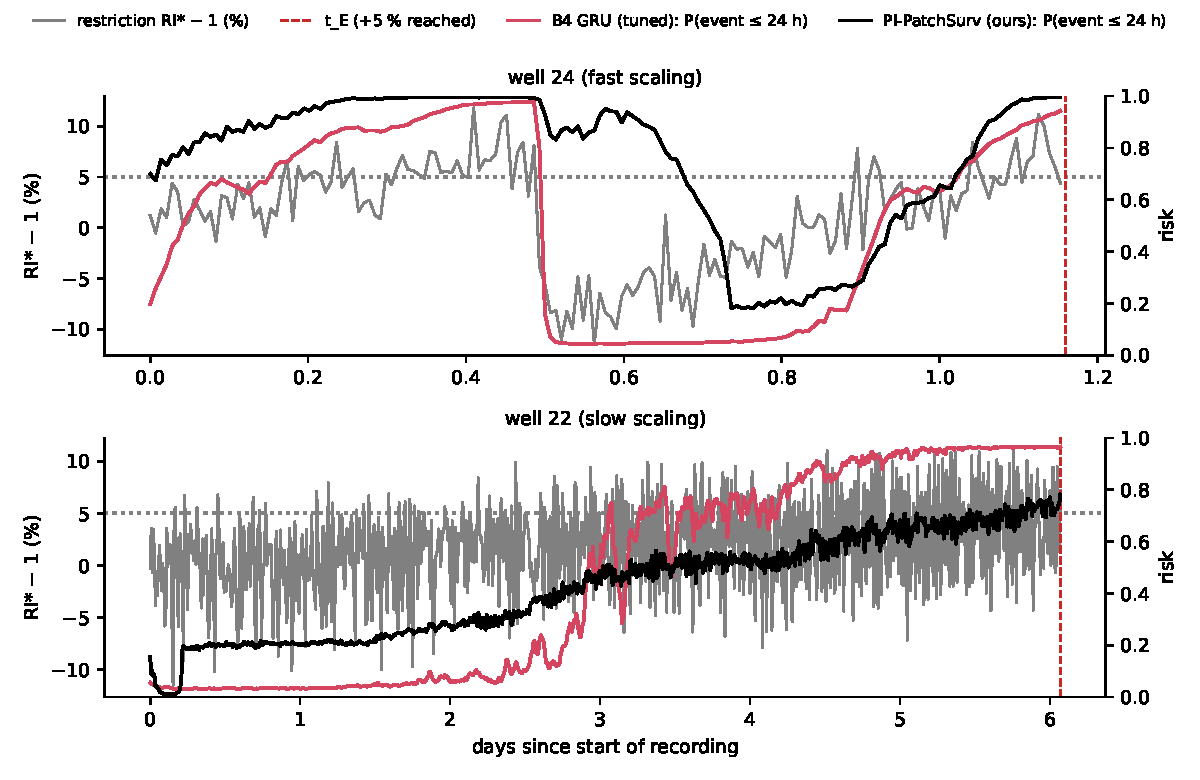
\includegraphics[width=\textwidth]{figures/example_forecasts.pdf}
\caption{Qualitative examples on two unseen test wells: the restriction $\RI-1$ (grey, left axis), the
critical level $+5\,\%$ (dotted) and the forecast risk of an event within 24~h (right axis) of the tuned GRU
and of PI-PatchSurv; the dashed red line marks $t_E$.}
\label{fig:examples}
\end{figure*}
